\subsection{Problem A1}\label{sec:qa1}\hfill

\begin{figure}[ht]
    \centering
    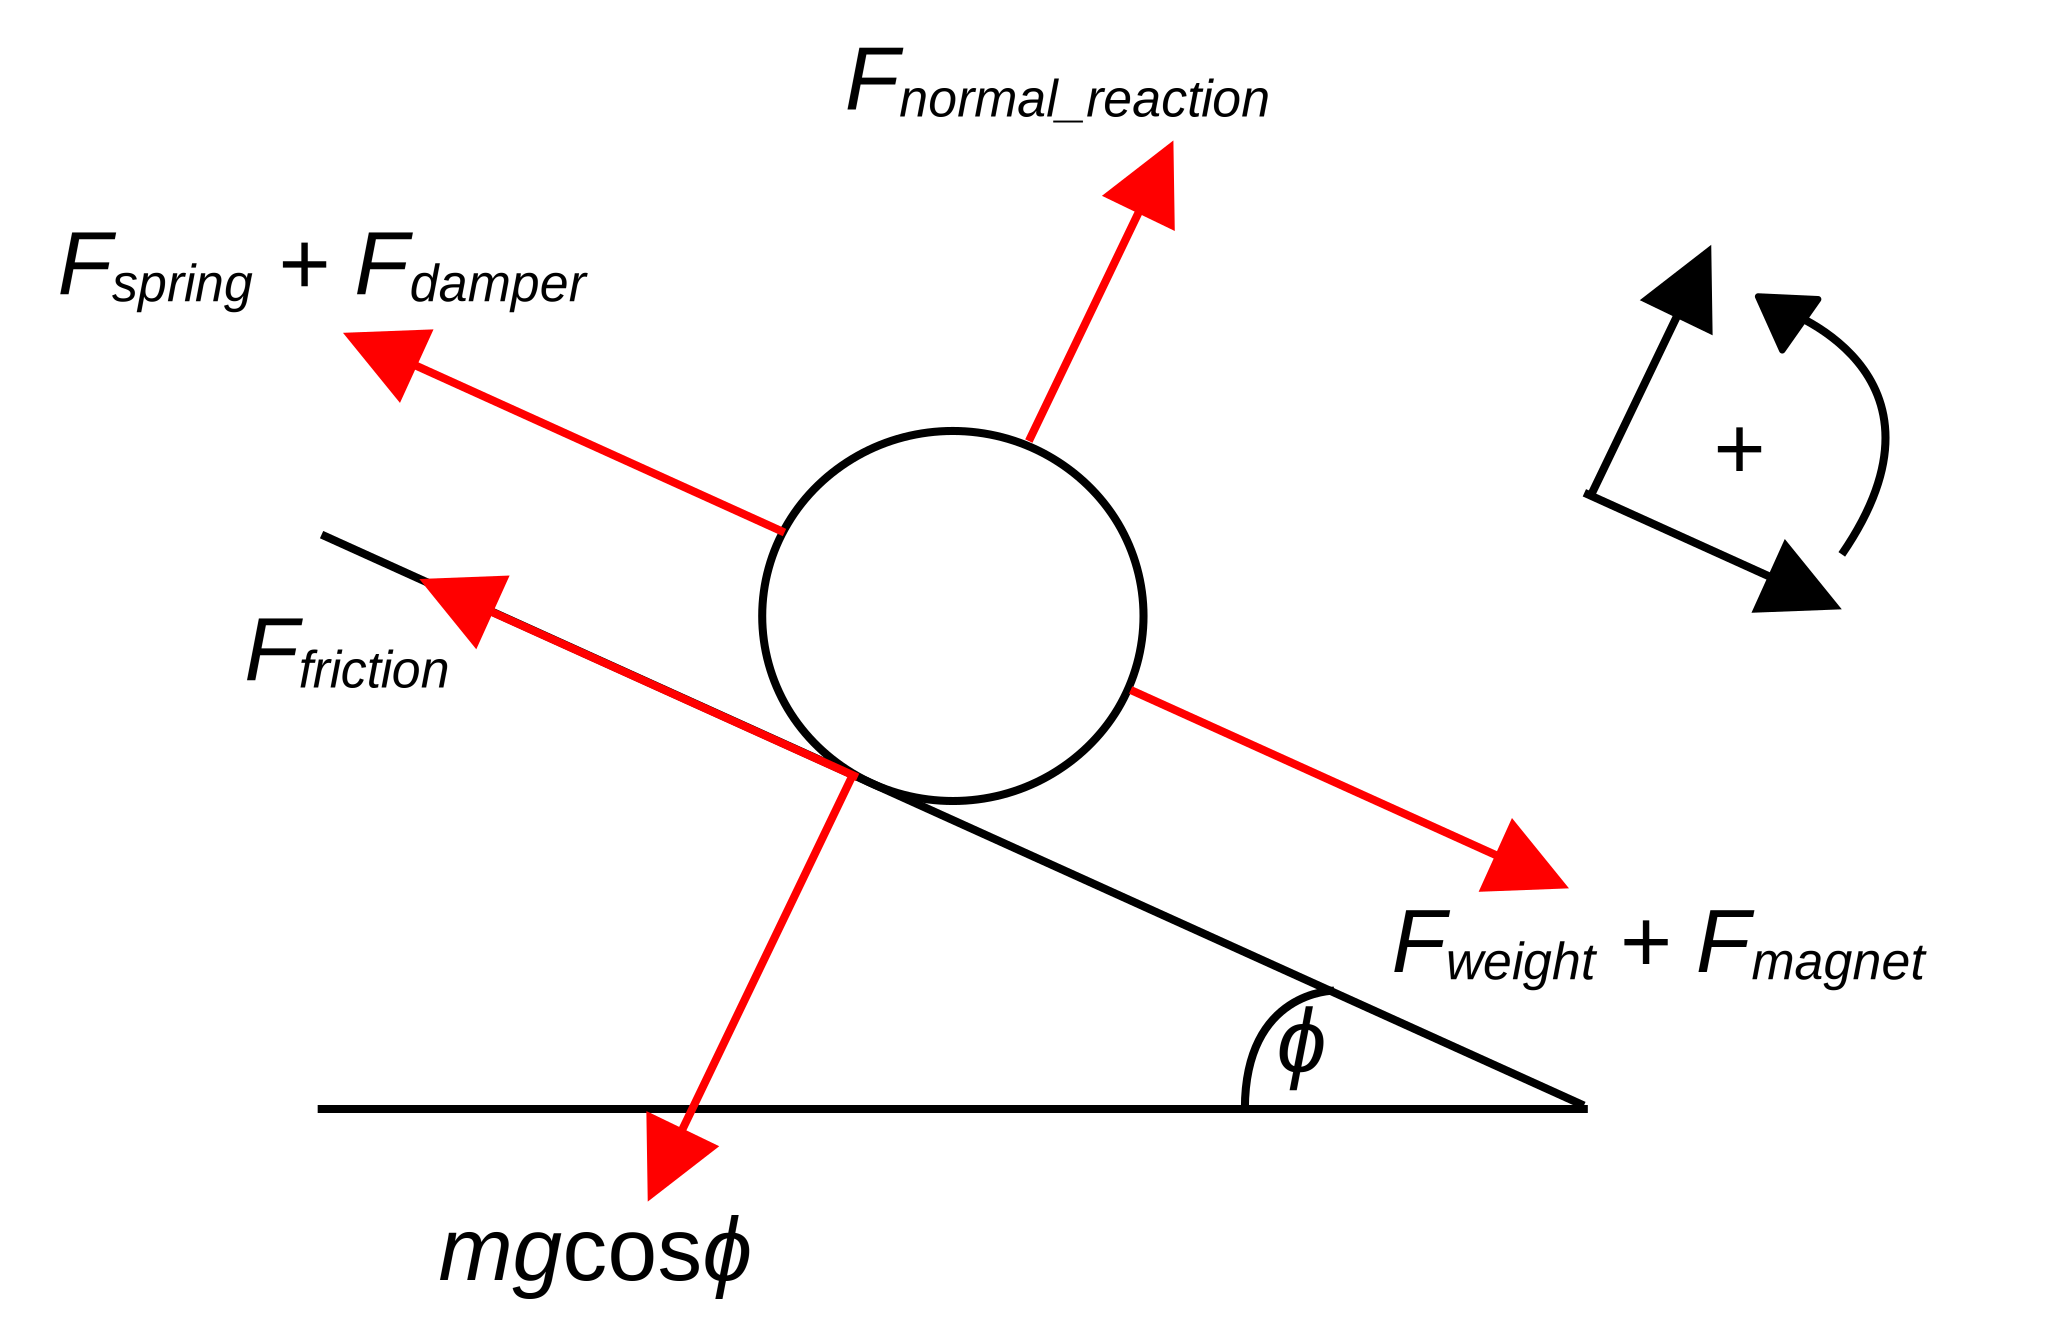
\includegraphics[width=0.45\linewidth]{forces_diagram}
    \caption{Diagram showing forces acting on the system and the inertial frame of reference.} \vspace{-2mm}
    \label{fig:forces_diagram}
\end{figure}
\begin{equation} \label{a1:total_0}
    F_{total} = F_{weight} + F_{magnet} - F_{spring} - F_{damper} - F_{friction}
\end{equation}
\begin{flalign} \label{a1:total_1}
    \text{The total force, } F_{total} = m\ddot{x}&&
\end{flalign}
\begin{flalign} \label{a1:weight}
    \text{The component of the weight acting down the plane, } F_{weight} = mg\sin \phi &&
\end{flalign}
\begin{flalign} \label{a1:spring}
    \text{The force of the spring, } F_{spring} = k \left( x - d \right)&&
\end{flalign}
\begin{flalign} \label{a1:damper}
    \text{The force of the damper, } F_{damper} = b \dot{x}&&
\end{flalign}
\begin{flalign} \label{a1:friction_0}
    \text{The force of friction, } F_{friction} r = - I_{inertia} \ddot{\theta}&&
\end{flalign}
\begin{flalign} \label{a1:theta_double_dot}
    \text{From the ``Pizza Slice Theorem'', } \ddot{\theta} = -\frac{\ddot{x}}{r}&&
\end{flalign}
\begin{flalign} \label{a1:friction_1}
    \text{Inertia of a solid sphere, } &I_{inertia} = \frac{2}{5}mr^2 \\
    \Longrightarrow &F_{friction} r = \frac{2}{5}mr^2 \frac{\ddot{x}}{r} \cr
    &F_{friction} = \frac{2}{5}m \ddot{x}&&
\end{flalign}
\begin{flalign} \label{a1:magnet}
    \text{The force of the magnet, } F_{magnet} = c \frac{I^2}{y^2}&&
\end{flalign}
\begin{flalign} \label{a1:y}
    \text{The distance, } y = \delta - x&&
\end{flalign}
\begin{flalign} \label{a1:current_dot}
    \text{The voltage, } &V = IR + \dot{I}L\cr
    \Longrightarrow &\dot{I} = \frac{1}{L} \left(V - IR \right)&&
\end{flalign}
\begin{flalign} \label{a1:inductance}
    \text{The inductance, } L = L_0 + L_1 e^{-\alpha y}&&
\end{flalign}
\noindent Substitute equations \eqref{a1:total_1} through \eqref{a1:inductance} into equation \eqref{a1:total_0}:
\begin{align} \label{a1:solution}
    m\ddot{x} &=
    mg\sin \phi
    + c \frac{I^2}{ \left( \delta - x \right)^2 }
    - k \left( x - d \right)
    - b \dot{x}
    - \frac{2}{5}m \ddot{x} \cr
    \ddot{x} &=
    \left( \frac{5}{7m} \right)
    \left( mg\sin \phi
    + c \frac{I^2}{ \left( \delta - x \right)^2 }
    - k \left( x - d \right)
    - b \dot{x} \right)
\end{align}